\documentclass[11pt,a4paper]{article}

% ---------------------------------------------------------------- packages --
\usepackage[utf8]{inputenc}
\usepackage[T1]{fontenc}
\usepackage[margin=1in]{geometry}
\usepackage{amsmath,amssymb}
\usepackage{graphicx}
\usepackage{booktabs}
\usepackage{longtable}
\usepackage{array}
\usepackage{listings}
\usepackage{xcolor}
\usepackage{caption}
\usepackage[hidelinks]{hyperref}

\graphicspath{{../../docs/mindmaps/}{../../docs/screenshots/}}

% ------------------------------------------------------------- listing style -
\definecolor{codegray}{gray}{0.95}
\definecolor{codegreen}{rgb}{0.0,0.5,0.0}
\definecolor{codeblue}{rgb}{0.1,0.1,0.6}
\lstdefinestyle{pseudo}{
  basicstyle=\ttfamily\small,
  backgroundcolor=\color{codegray},
  frame=single, framerule=0pt, breaklines=true,
  columns=fullflexible, keepspaces=true,
  xleftmargin=6pt, xrightmargin=6pt, aboveskip=6pt, belowskip=6pt,
}
\lstdefinestyle{py}{
  language=Python, style=pseudo,
  keywordstyle=\color{codeblue}\bfseries,
  commentstyle=\color{codegreen}\itshape,
  stringstyle=\color{purple},
  numbers=left, numberstyle=\tiny\color{gray}, numbersep=6pt,
}

\newcolumntype{L}[1]{>{\raggedright\arraybackslash}p{#1}}

% ----------------------------------------------------------------- metadata --
\title{\textbf{SOEN 6011 --- Deliverable 1}\\[2pt]
       \large Function F6: The Real Beta Function $B(x,y)$\\
       Persona, Requirements, Algorithms, and a Command-Line Prototype}
\author{SOEN 6011 --- Software Engineering Processes}
\date{2026-07-15}

\begin{document}
\maketitle

\begin{abstract}
\noindent This report documents Deliverable 1 for Function F6, the real Beta
function $B(x,y)=\int_0^1 t^{x-1}(1-t)^{y-1}\,dt$ scoped to $x>0,\,y>0$. It presents
a goal-directed user persona (Problem~1), a requirements specification aligned with
ISO/IEC/IEEE~29148 (Problem~2), two genuinely different language-neutral algorithms
(Problem~3), and the selection of one algorithm together with a runnable Python
command-line prototype (Problem~4). Each problem was supported by a documented
generative-AI (GAI) prompt using the CASTROFF framework; every AI output was
critically evaluated and independently verified against trusted reference values.
The delivered prototype meets its accuracy requirement with a worst-case relative
error of $1.17\times10^{-14}$, eight orders of magnitude inside the $10^{-6}$
tolerance.
\end{abstract}

\tableofcontents
\bigskip

% ============================================================================
\section{Introduction and scope}
The assigned function is the real Beta function
\[
  B(x,y)=\int_0^1 t^{x-1}(1-t)^{y-1}\,dt
        =\frac{\Gamma(x)\,\Gamma(y)}{\Gamma(x+y)},
  \qquad B(x,y)=B(y,x).
\]
Following decision~D-001 the supported domain is restricted to $x>0,\,y>0$, where the
Euler integral is finite and real; analytic continuation, complex arguments, and the
incomplete Beta function are out of scope for D1. Reference definitions and properties
are taken from the NIST DLMF~\cite{dlmf512} and Abramowitz \&
Stegun~\cite{abramowitz1964handbook}.

All work is version-tracked in the repository \texttt{beta-function-calculator/}, whose
\texttt{docs/} tree contains the research notes, decision log, GAI prompt log, and the
per-problem artifacts referenced throughout this report.

% ============================================================================
\section{Problem 1 --- Persona}
\label{sec:p1}

\subsection{Approach and template selection}
Three persona-template styles were compared --- goal-directed
(Cooper~\cite{cooper2004inmates}), role-based, and proto/lightweight --- against five
criteria: relevance to a computation tool, realism, conciseness, traceability to
requirements, and accessibility support. The goal-directed template was chosen because
it centres user \emph{goals and pain points}, which gives the strongest traceability
into later requirements; the explicit evidence/assumption labelling of proto personas
was grafted on (decision~D-005). Figure~\ref{fig:personamap} shows the selection
mind map.

\begin{figure}[htbp]
  \centering
  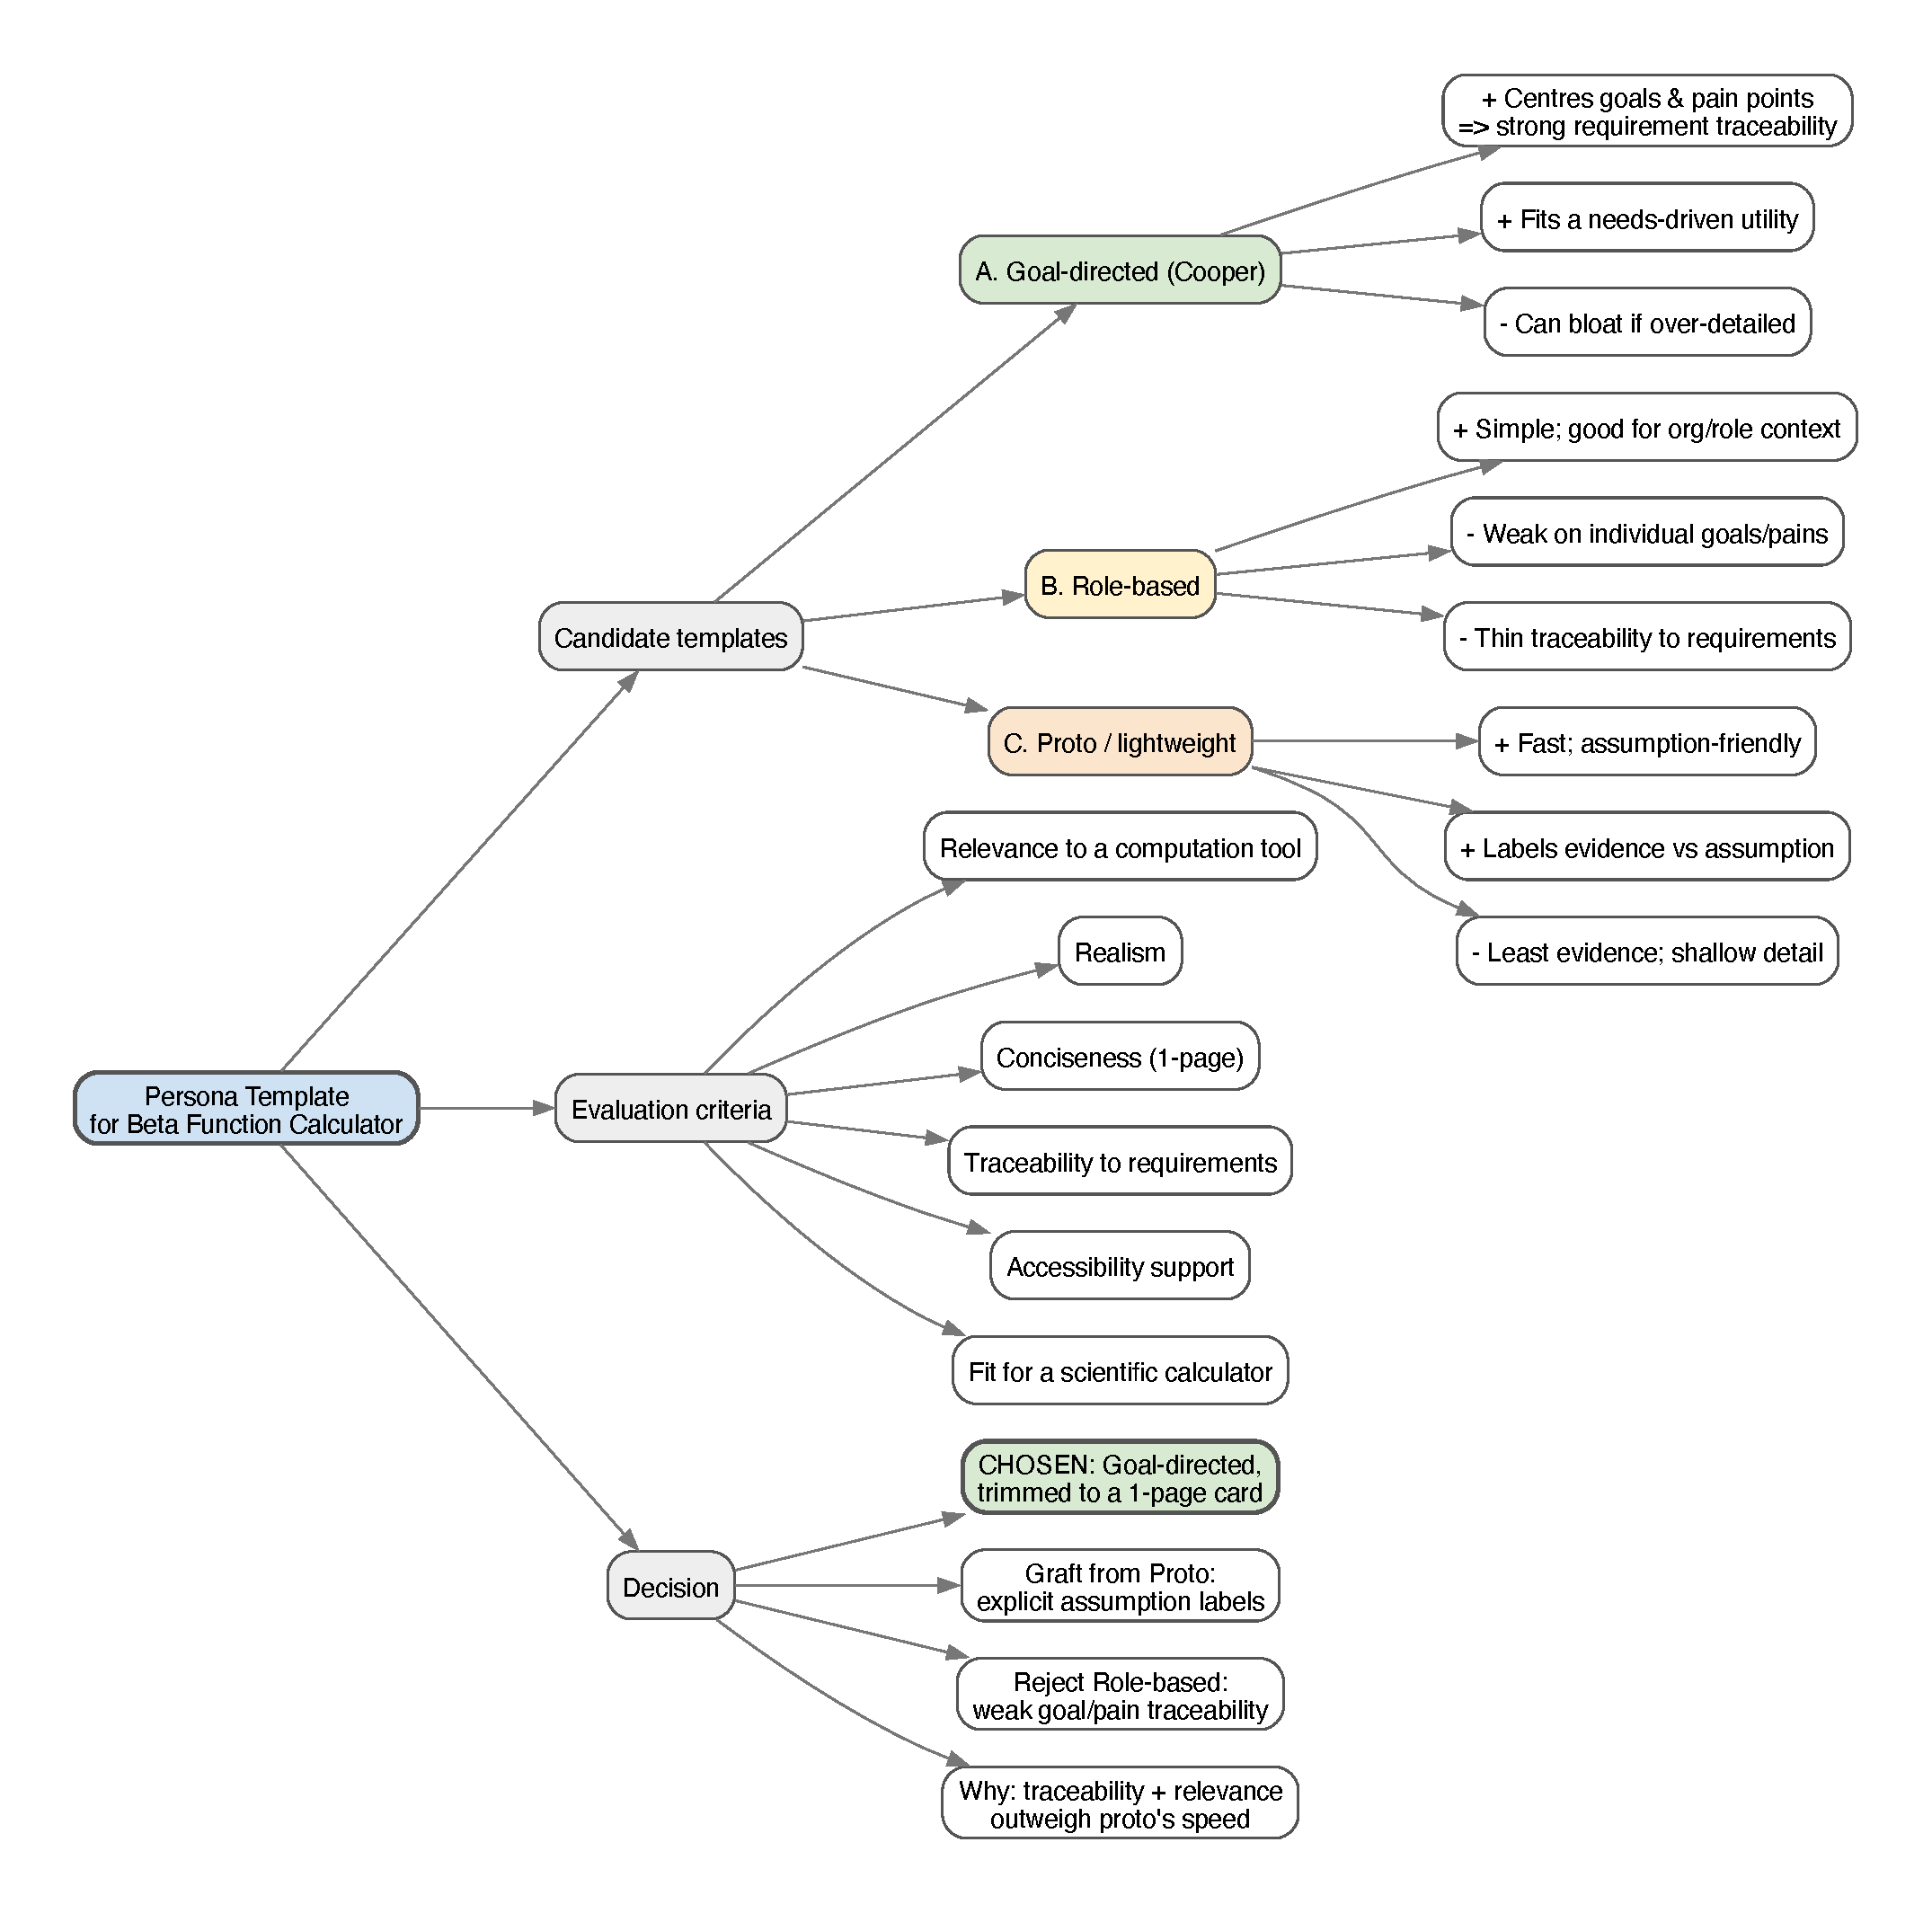
\includegraphics[width=0.95\textwidth]{persona_template_selection.pdf}
  \caption{Persona-template selection mind map (Problem~1). Meaning is carried by text
           labels, not colour alone, for accessibility.}
  \label{fig:personamap}
\end{figure}

\subsection{The persona}
The resulting primary persona is \textbf{Maya Fernandes}, an MSc Statistics student and
part-time research assistant who is strong in mathematics but has low comfort with
special-function libraries and the command line. Her goals are: obtain a quick,
trustworthy $B(x,y)$ value without writing code (G1); verify coursework (G2); and
understand which inputs are valid (G3). Her pain points include uncertainty about the
valid input range (N1), cryptic errors or wrong \texttt{inf} values from existing tools
(N2), a desire for honestly stated precision (N3), low CLI comfort (N4), occasional
screen-reader use (N5), and unwillingness to install a library for a single value (N6).
Attributes are tagged \textbf{[E]} evidence, \textbf{[S]} synthesis, or \textbf{[A]}
assumption; the persona is explicitly synthesised, not an interviewed individual.

\subsection{GAI use and critical evaluation}
\textbf{Tool:} Claude (Opus~4.8) via Claude Code. \textbf{Prompt type:} generative +
decision-support. The CASTROFF prompt asked for a comparison of $\ge 3$ persona templates
against stated criteria, then a goal-directed persona for a Beta-function user, with
strict evidence/assumption labelling and a ban on invented statistics or irrelevant
biography (excerpt):
\begin{quote}\small\itshape
``First, compare at least three established persona-template styles \ldots\ recommend which
single template is most suitable \ldots\ Then, using the recommended template, draft one
realistic primary persona \ldots\ Clearly separate what is evidence, what is reasonable
synthesis, and what is an explicit assumption.''
\end{quote}
\textbf{Accepted:} the goal-directed recommendation and the needs$\rightarrow$requirements
mapping. \textbf{Adjusted:} age, education, and screen-reader use were retagged as
explicit assumptions~[A]. \textbf{Verification:} every pain point was cross-checked
against the domain research (applications and numerical risks), and the traceability gate
(seven needs mapping to requirements, $\ge 5$ required) was confirmed satisfied.

% ============================================================================
\section{Problem 2 --- Requirements (ISO/IEC/IEEE 29148)}
\label{sec:p2}

Requirements follow the 29148 imperative pattern
(\emph{[condition] the system shall [action] [object] [constraint]}), each statement
singular and verifiable, with category-prefixed identifiers and a planned verification
method (T~test, I~inspection, A~analysis, D~demonstration)~\cite{iso29148}. The baseline
was frozen at v0.1 after a seven-characteristic quality review. Table~\ref{tab:reqs}
lists the requirements; assumptions are recorded separately.

\begin{longtable}{L{1.4cm} L{8.2cm} L{1.0cm} L{1.2cm}}
  \caption{Requirements baseline v0.1 (abbreviated statements).}\label{tab:reqs}\\
  \toprule
  \textbf{ID} & \textbf{Requirement (shall)} & \textbf{Pri} & \textbf{Verify}\\
  \midrule
  \endfirsthead
  \toprule
  \textbf{ID} & \textbf{Requirement (shall)} & \textbf{Pri} & \textbf{Verify}\\
  \midrule
  \endhead
  FR-01  & Accept two real inputs $x$ and $y$. & M & D\\
  FR-02  & Compute $B(x,y)$ for valid inputs. & M & T\\
  FR-03  & Display the numeric result. & M & D\\
  FR-04  & Allow another calculation without restarting. & M & D\\
  FR-05  & Provide a command to exit. & M & D\\
  VAL-01 & Reject $x\le 0$ or $y\le 0$ (no computation). & M & T\\
  VAL-02 & Reject non-numeric input. & M & T\\
  VAL-03 & Reject empty input and re-prompt. & M & T\\
  VAL-04 & Reject magnitude $>10^4$ with a range message. & S & T\\
  ACC-01 & Relative error $\le 10^{-6}$ vs.\ reference over $0<x,y\le 50$. & M & T\\
  ACC-02 & Display to 6 significant figures; no false precision. & M & I\\
  REL-01 & No unhandled exception on any supported input. & M & T\\
  REL-02 & No non-finite (\texttt{inf}/\texttt{nan}) result when finite. & M & T\\
  REL-03 & Terminate within bounded work. & M & A\\
  PERF-01& Return within 1\,s on a typical laptop. & S & T\\
  USE-01 & Plain-language prompts stating the valid domain. & M & I\\
  USE-02 & Concise usage instructions available. & S & I\\
  ERR-01 & Specific message: what was wrong and how to fix. & M & T\\
  ACC-03 & Convey status/errors by text, not colour alone. & S & I\\
  POR-01 & Run from a terminal via Python~3, no IDE. & M & D\\
  DOC-01 & Document supported domain and assumptions in help. & S & I\\
  \bottomrule
\end{longtable}

\noindent\textbf{Key assumptions:} domain $x,y>0$ (A-01, D-001); real decimal I/O
(A-02); magnitude cap $10^4$ (A-04); accuracy target $10^{-6}$ over $0<x,y\le 50$
(A-05, D-007). The quality review resolved vague terms (quantified ACC-01/PERF-01/ERR-01),
split a compound ``compute and display'' statement into FR-02/FR-03, and closed an
accessibility gap by adding ACC-03.

\subsection{GAI use and critical evaluation}
\textbf{Tool:} Claude (Opus~4.8). \textbf{Prompt type:} transformational (persona needs
$\rightarrow$ verifiable requirements) + review. The CASTROFF prompt supplied the finalised
persona and required 29148-style statements, a category-prefixed ID scheme, priorities,
verification methods, a separate assumptions list, and a quality-review pass; it forbade
prescribing any algorithm or library and banned unquantified terms such as ``fast''.
\textbf{Accepted:} the ID scheme, the quantified $10^{-6}$ tolerance, and the FR-02/FR-03
split. \textbf{Adjusted:} the numeric bounds (A-04/A-05/PERF-01) were flagged as
assumptions to re-validate after the D2 from-scratch build. \textbf{Verification:} each
requirement was checked for singularity and a verification method; the potential
REL-02/ACC-01 conflict for huge inputs was resolved by the VAL-04 cap.

% ============================================================================
\section{Problem 3 --- Two algorithms}
\label{sec:p3}

Two substantially different, language-neutral algorithms were specified.

\subsection{Algorithm A --- Euler-integral adaptive quadrature}
Algorithm~A approximates $B(x,y)=\int_0^1 t^{x-1}(1-t)^{y-1}dt$ directly with adaptive
Simpson's rule, insetting singular endpoints and capping recursion depth for guaranteed
termination.

\begin{lstlisting}[style=pseudo]
function BETA_QUADRATURE(x, y, tol, maxDepth)
    if x <= 0 or y <= 0 then error DomainError        # VAL-01
    function f(t)                                      # integrand
        if t <= 0 or t >= 1 then return 0
        return t^(x-1) * (1-t)^(y-1)
    lo <- (EPS if x < 1 else 0)                        # inset singular ends
    hi <- (1 - EPS if y < 1 else 1)
    return ADAPT(f, lo, hi, tol, SIMPSON(f, lo, hi), 0, maxDepth)

function SIMPSON(f, a, b)
    c <- (a + b) / 2
    return (b - a) / 6 * (f(a) + 4*f(c) + f(b))

function ADAPT(f, a, b, tol, whole, depth, maxDepth)
    c <- (a + b) / 2
    left  <- SIMPSON(f, a, c);  right <- SIMPSON(f, c, b)
    if depth >= maxDepth or |left + right - whole| <= 15*tol then  # stop / REL-03
        return left + right + (left + right - whole) / 15          # Richardson
    return ADAPT(f, a, c, tol/2, left,  depth+1, maxDepth)
         + ADAPT(f, c, b, tol/2, right, depth+1, maxDepth)
\end{lstlisting}
\noindent\textbf{Complexity} $O(N)$ integrand evaluations (bounded by \texttt{maxDepth}).
\textbf{Verified weakness:} for strong endpoint singularities it loses accuracy ---
$B(0.2,0.3)$ returns $7.72774$ vs.\ the true $7.74848$, a relative error $\approx
2.7\times10^{-3}$ that \emph{fails ACC-01}.

\subsection{Algorithm B --- Gamma identity via Lanczos $\ln\Gamma$ (log domain)}
Algorithm~B uses $B(x,y)=\Gamma(x)\Gamma(y)/\Gamma(x+y)$ evaluated in the log domain,
$B=\exp(\ln\Gamma(x)+\ln\Gamma(y)-\ln\Gamma(x+y))$, with a Lanczos $\ln\Gamma$
approximation~\cite{lanczos1964gamma,press2007numerical}. The log domain avoids Gamma
overflow (REL-02) and the fixed-length Lanczos loop guarantees termination (REL-03).

\begin{lstlisting}[style=pseudo]
function BETA_GAMMA(x, y)
    if x <= 0 or y <= 0 then error DomainError                     # VAL-01
    return EXP( LN_GAMMA(x) + LN_GAMMA(y) - LN_GAMMA(x + y) )

function LN_GAMMA(z)                                # z > 0, Lanczos g = 7
    if z < 0.5 then                                 # reflection for small args
        return LN(pi) - LN(|SIN(pi*z)|) - LN_GAMMA(1 - z)
    z <- z - 1;  a <- P[0]
    for i <- 1 to g + 1 do   a <- a + P[i] / (z + i)   # fixed loop -> REL-03
    t <- z + g + 0.5
    return 0.5*LN(2*pi) + (z + 0.5)*LN(t) - t + LN(a)
\end{lstlisting}
\noindent\textbf{Complexity} $O(1)$ --- a constant number of terms (satisfies PERF-01).
\textbf{Weakness:} accuracy is bounded by the Lanczos coefficient set ($\approx 15$
significant digits at $g=7$).

\subsection{How the two differ, and verification}
The algorithms are genuinely different: A \emph{integrates the definition numerically};
B \emph{evaluates a closed-form identity via a series approximation}. They share only
basic arithmetic. Both were implemented and compared to \texttt{math.lgamma} across eight
cases (integer, half-integer, large, and near-singular): B matches to $\sim 10$ digits
everywhere, whereas A degrades near the singular corner as noted above. This empirical
evidence directly drives the Problem~4 selection.

\subsection{GAI use and critical evaluation}
\textbf{Tool:} Claude (Opus~4.8). \textbf{Prompt type:} generative + comparative. The
CASTROFF prompt supplied the relevant requirement IDs and required two textbook-style
pseudocode listings with pre/postconditions, termination safeguards, complexity,
weaknesses, and worked traces, in language-neutral form (no Python syntax).
\textbf{Accepted:} both listings and the comparison table. \textbf{Verified independently:}
rather than trusting the output, both algorithms were coded and checked against
\texttt{math.lgamma}; the discovery that A fails ACC-01 near singular endpoints was the
decisive, self-generated evidence for Problem~4.

% ============================================================================
\section{Problem 4 --- Selection and CLI prototype}
\label{sec:p4}

\subsection{Selection}
Figure~\ref{fig:algmap} compares the two algorithms against accuracy, domain coverage,
numerical stability, implementation effort, fitness for the D2 from-scratch build,
performance, and explainability. \textbf{Algorithm~B was selected} (decision~D-004): it
is the only candidate meeting ACC-01 uniformly across the domain \emph{and} REL-02
(log-domain, no overflow), REL-03 (fixed loop), and PERF-01 ($O(1)$). Algorithm~A was
rejected for this stage because it fails ACC-01 near the singular corner. The trade-off
accepted is that B requires slightly more from-scratch effort in D2 ($\exp$, $\ln$,
$\sin$); this is justified because accuracy is a must-have requirement whereas A's
intuitiveness is not.

\begin{figure}[htbp]
  \centering
  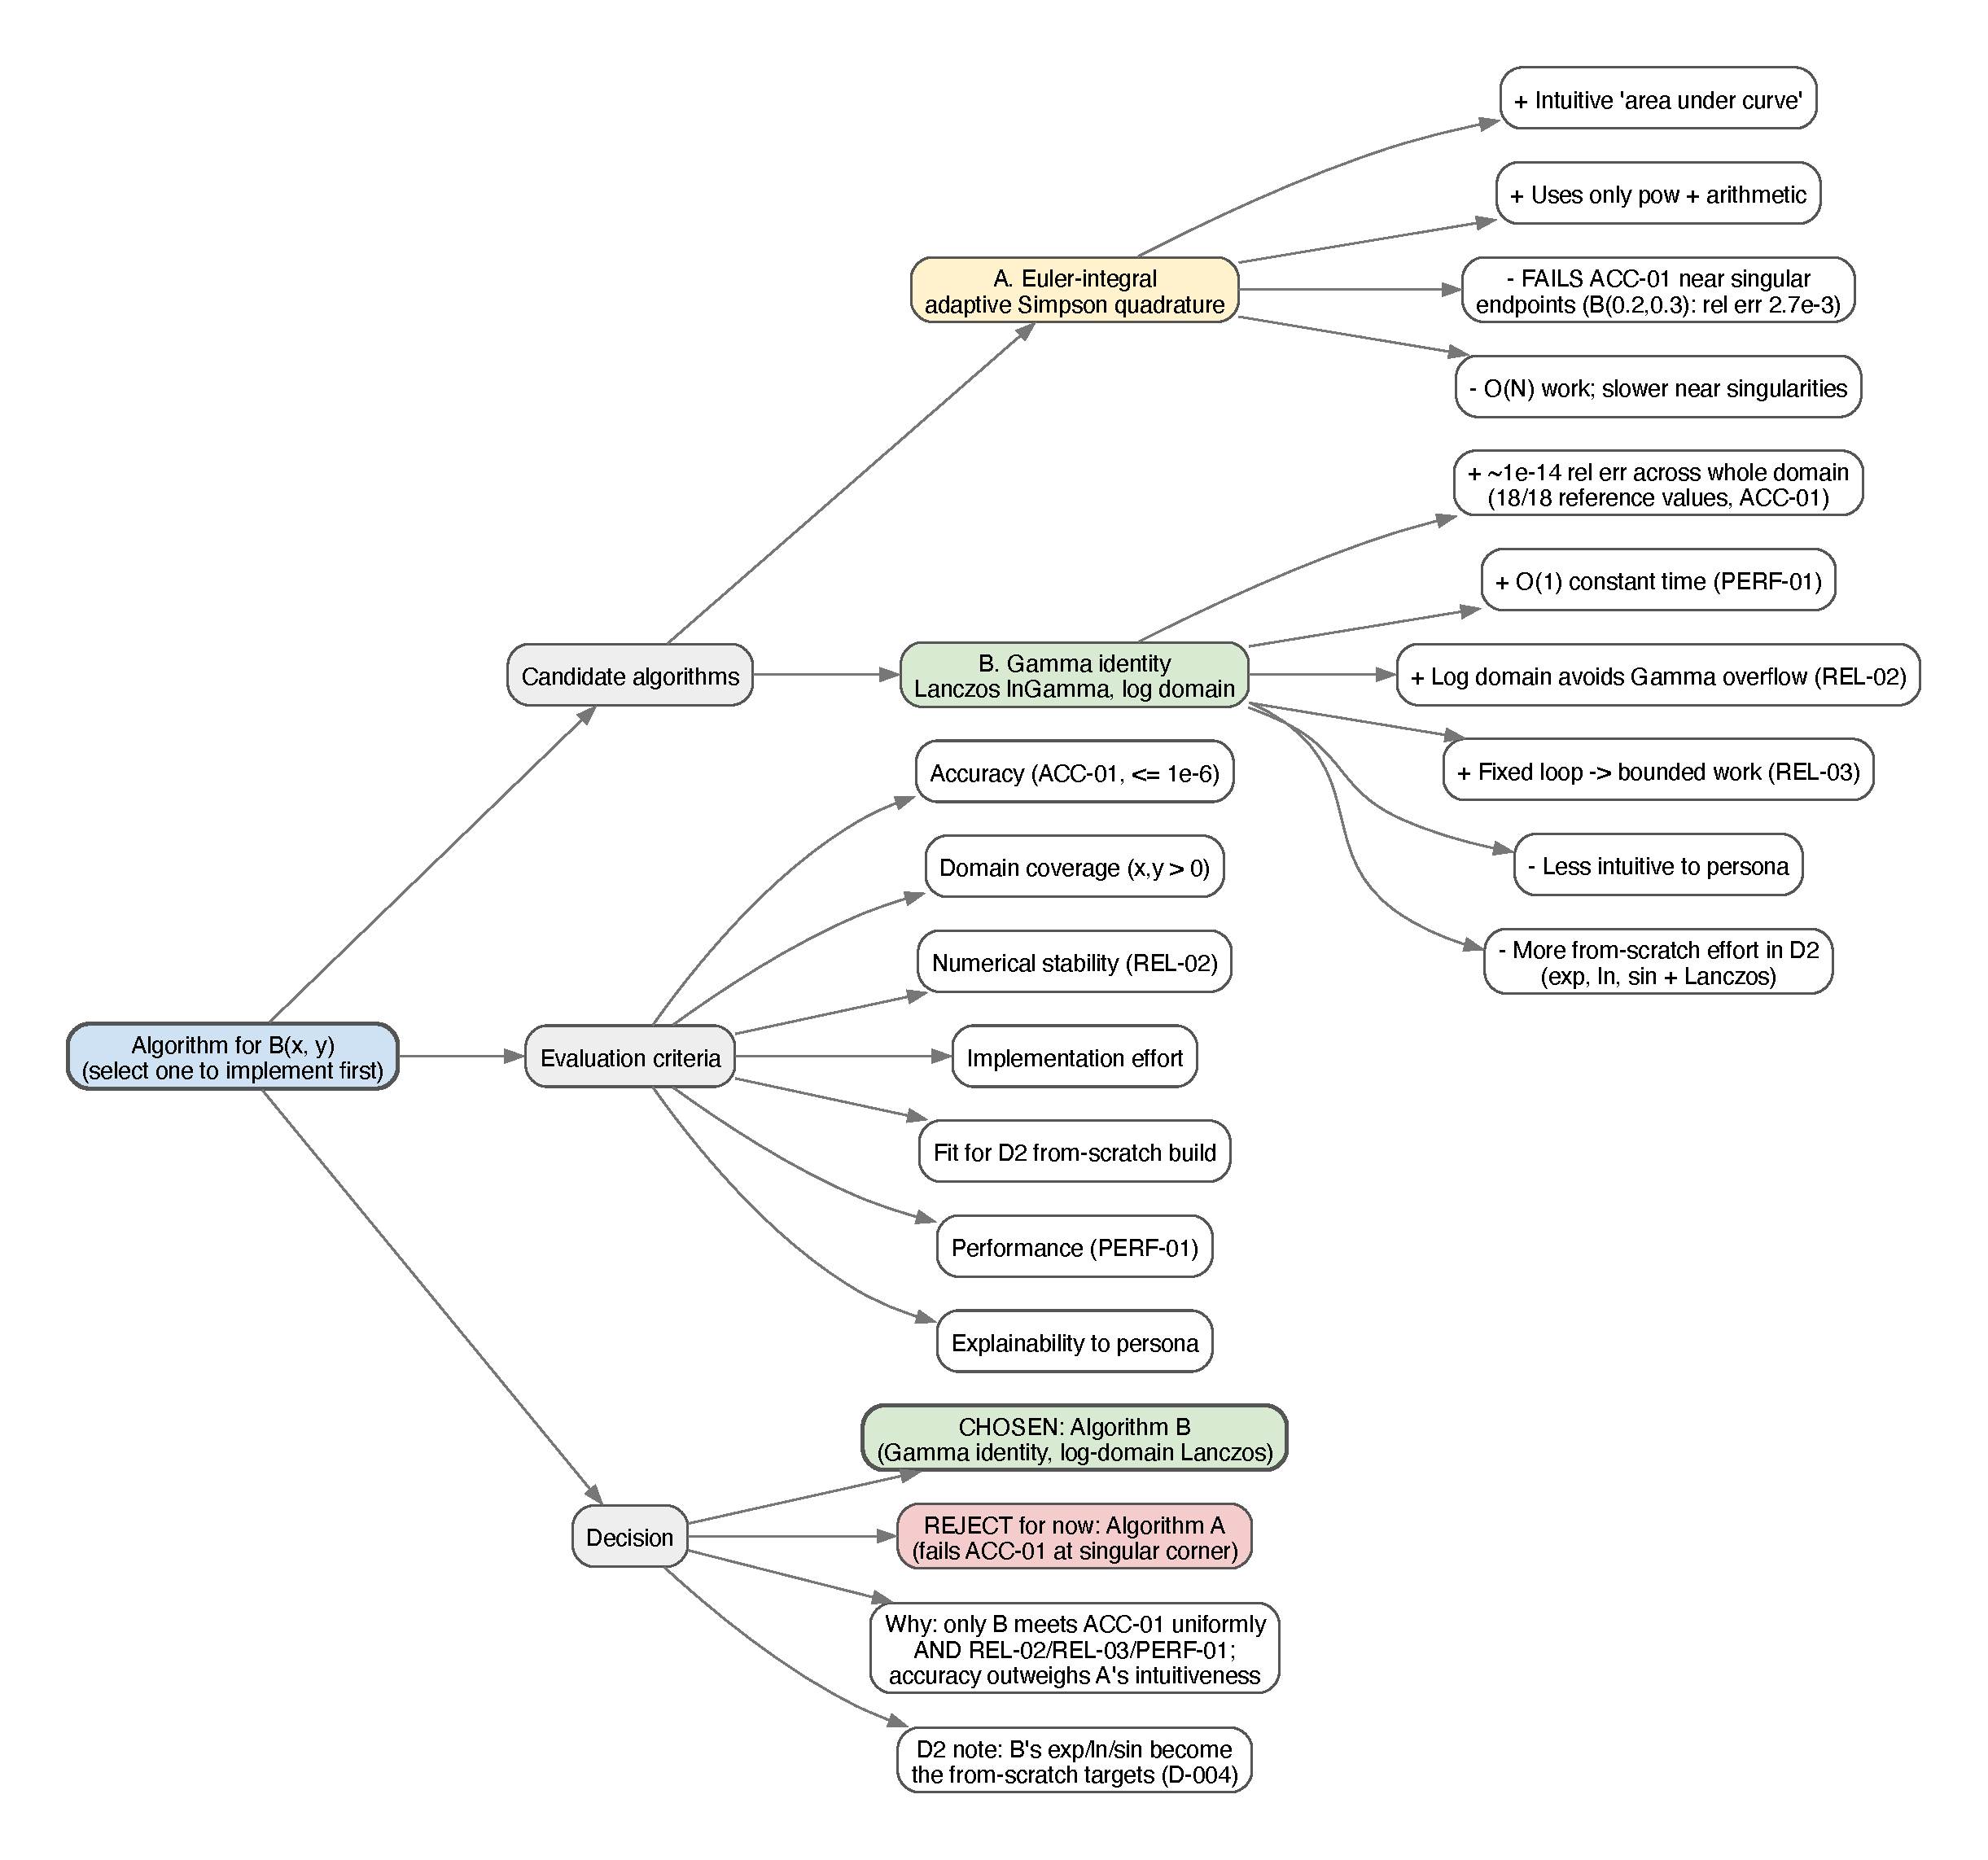
\includegraphics[width=\textwidth]{algorithm_selection.pdf}
  \caption{Algorithm-selection mind map (Problem~4). The decision follows from the
           verified evidence, not preference.}
  \label{fig:algmap}
\end{figure}

\subsection{Implementation}
The prototype \texttt{src/cli.py} separates a pure computation core
(\texttt{beta}, \texttt{beta\_ln}, \texttt{ln\_gamma}) from a console I/O layer, so the
core is independently testable and reusable by the D2 GUI. Input is validated for
emptiness, non-numeric text, non-positivity, and over-cap magnitude, each with a specific
message; results are shown to six significant figures. The core listing:

\begin{lstlisting}[style=py]
def ln_gamma(z):
    """Natural log of Gamma(z) via the Lanczos approximation (g = 7)."""
    if z < 0.5:                       # reflection keeps precision for small z
        return math.log(math.pi / math.sin(math.pi * z)) - ln_gamma(1.0 - z)
    z -= 1.0
    a = _LANCZOS_P[0]
    for i in range(1, _LANCZOS_G + 2):        # fixed-length loop -> REL-03
        a += _LANCZOS_P[i] / (z + i)
    t = z + _LANCZOS_G + 0.5
    return 0.5*math.log(2.0*math.pi) + (z + 0.5)*math.log(t) - t + math.log(a)

def beta(x, y):
    """Real Beta B(x, y) for x > 0, y > 0 (Algorithm B); finite, O(1)."""
    if x <= DOMAIN_MIN or y <= DOMAIN_MIN:
        raise ValueError("domain is x > 0 and y > 0")
    return math.exp(beta_ln(x, y))            # log domain avoids overflow (REL-02)
\end{lstlisting}

\noindent\textbf{D2 from-scratch note.} This D1 prototype borrows only the elementary
primitives \texttt{math.log}, \texttt{math.exp}, \texttt{math.sin}, and the constant
$\pi$; it deliberately does \emph{not} call \texttt{math.gamma}/\texttt{lgamma}/
\texttt{beta}. Those three functions are the entire from-scratch obligation for
Deliverable~2 --- the Lanczos series and log-domain combination are already hand-written.

\subsection{Sample runs}
Figures~\ref{fig:valid}--\ref{fig:invalid} are genuine terminal transcripts (captured
through a pseudo-terminal so typed input is echoed). Valid, boundary/near-singular, and
invalid cases all behave correctly, and no invalid input produces an unhandled traceback.

\begin{figure}[htbp]
  \centering
  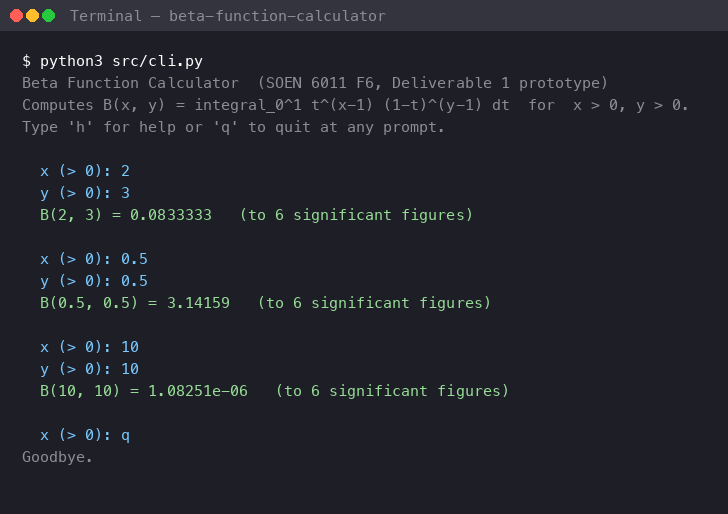
\includegraphics[width=0.82\textwidth]{run_valid.png}
  \caption{Valid cases: $B(2,3)$, $B(0.5,0.5)=\pi$, and $B(10,10)$.}
  \label{fig:valid}
\end{figure}
\begin{figure}[htbp]
  \centering
  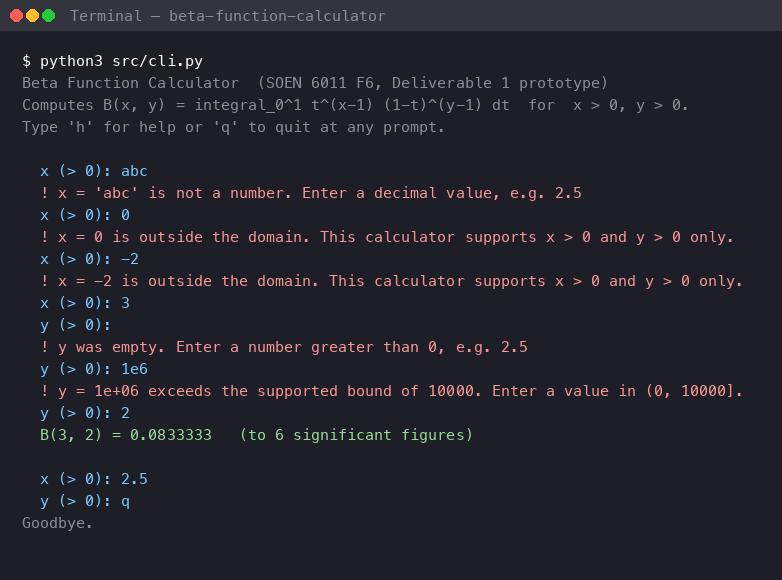
\includegraphics[width=0.82\textwidth]{run_invalid.png}
  \caption{Invalid cases: non-numeric, zero, negative, empty, and over-cap inputs are each
           rejected with a specific message instead of crashing (REL-01, ERR-01).}
  \label{fig:invalid}
\end{figure}

\subsection{GAI use and critical evaluation}
\textbf{Tool:} Claude (Opus~4.8). \textbf{Prompt type:} decision-support (selection mind
map) + generative (Python CLI). The CASTROFF prompt supplied both Problem~3 algorithms and
required an evidence-based selection followed by a terminal program with I/O separated from
computation, robust validation, and documented precision, while noting which \texttt{math}
calls would need from-scratch replacement in D2. \textbf{Accepted:} the selection of B ---
the only candidate meeting ACC-01 uniformly. \textbf{Adjusted:} $\ln\Gamma$ was implemented
by hand via Lanczos rather than calling \texttt{math.lgamma}, so the D2 obligation is
honest and narrowly scoped. \textbf{Rejected:} any library \texttt{gamma}/\texttt{beta}
call, and any colour-only status output (ACC-03). \textbf{Verification:} see
Section~\ref{sec:verify}.

% ============================================================================
\section{Verification and known limitations}
\label{sec:verify}

A re-runnable harness (\texttt{tests/verify\_d1.py}) exercises every machine-checkable
requirement and passes \textbf{15/15}. Highlights: ACC-01 holds across all 18 trusted
reference values with a worst relative error of $1.17\times10^{-14}$ (including the
$B(0.2,0.3)$ corner where Algorithm~A failed); REL-01 shows zero crashes across ten
malformed inputs; REL-02 returns finite values for all 36 large/small supported inputs;
and PERF-01 measures $\approx 1.3\,\mu\text{s}$ per computation, far inside the 1\,s
budget. A full requirement-by-requirement matrix is provided in
\texttt{docs/verification\_matrix.md}.

\paragraph{Known limitations (honest disclosure).} The domain is $x,y>0$ only (no analytic
continuation or complex arguments); magnitudes above $10^4$ are rejected by design;
accuracy is bounded by the Lanczos $g=7$ coefficient set and was validated against an
lgamma-based reference over $0<x,y\le 50$; and the prototype relies on \texttt{math}
primitives that D2 must reimplement. Each limitation is a documented scope boundary or
assumption (D-001/D-004/D-007, A-01/A-04/A-05/A-06), not a correctness defect within the
supported domain.

% ============================================================================
\section{Decision rationale summary}
The significant decisions are recorded in \texttt{docs/decisions/decision\_log.md}:
D-001 scopes the domain to $x,y>0$; D-005 selects the goal-directed persona template;
D-006 adopts the 29148 imperative ``shall'' style; D-007 sets the $10^{-6}$ tolerance and
$10^4$ magnitude cap; and D-004 selects Algorithm~B as the primary algorithm on the basis
of the verified accuracy evidence. Every GAI interaction is logged in
\texttt{docs/prompts/gai\_prompt\_log.md} with its prompt, an output summary, a critical
evaluation, and an independent verification note.

% ----------------------------------------------------------------- references
\bibliographystyle{ieeetr}
\bibliography{references}

\end{document}
